\documentclass{article}

% Packages
\usepackage{geometry}
\usepackage{graphicx}
\usepackage{lipsum}
\usepackage{listings}
\usepackage[portuguese]{babel}

% -- Defining colors:
\usepackage[dvipsnames]{xcolor}
\definecolor{codegreen}{rgb}{0,0.6,0}
\definecolor{codegray}{rgb}{0.5,0.5,0.5}
\definecolor{codepurple}{rgb}{0.58,0,0.82}
\definecolor{backcolour}{rgb}{0.95,0.95,0.92}

% Definig a custom style:
\lstdefinestyle{mystyle}{
    backgroundcolor=\color{backcolour},   
    commentstyle=\color{codepurple},
    keywordstyle=\color{NavyBlue},
    numberstyle=\tiny\color{codegray},
    stringstyle=\color{codepurple},
    basicstyle=\ttfamily\footnotesize\bfseries,
    breakatwhitespace=false,         
    breaklines=true,                                   
    keepspaces=true,                 
    numbers=left,                    
    numbersep=5pt,                  
    showspaces=false,                
    showstringspaces=false,
    showtabs=false,                  
    tabsize=2,
    captionpos=b
}

% -- Setting up the custom style:
\lstset{style=mystyle}

% Page setup
\geometry{a4paper, margin=2cm}

\begin{document}

% cover
\thispagestyle{empty} % Remove page number from first page

\begin{figure}[t]
    
\includegraphics[width=3cm]{images/logo-puc-minas.png}
    \hspace{0.02\textwidth}
    \vline%
    \hspace{0.04\textwidth}
    
\includegraphics[width=3cm]{images/logo-icei.jpeg}
\end{figure}

\hrulefill%
\vspace{\baselineskip}

\Large\noindent
\textbf{Pontifícia Universidade Católica de Minas Gerais} \\
\textbf{Instituto de Ciências Exatas e Informática} \\
\textbf{Departamento de Engenharia de Computação}

\begin{center}
    \vfill
    \Huge\textbf{Relatório: Trabalho Prático 2} \\
    \vspace{0.5cm}
    \Large\textbf{Registradores em VHDL} \\
    \vspace{1cm}
    \large \textbf{Professor(es)}: Antônio Hamilton Magalhães\\
    \vspace{0.5cm}
    \large \textbf{Aluno(s)}: Bruno Luiz Dias Alves de Castro \\
    \large \hspace{0.75cm} Rafael Ramos de Andrade \\
    \vfill
    \large Belo Horizonte \\ Campus Coração Eucarístico \\
    \vspace{\baselineskip}
    \large \today
\end{center}

% table of contents
\newpage
\thispagestyle{empty}
\tableofcontents

% body
\newpage
\large % document text size

\section{Introdução}

Durante as aulas da disciplina de Sistemas Reconfiguráveis, fomos introduzidos à linguagem VHDL. VHDL (\textbf{V}HSIC \textbf{H}ardware \textbf{D}escription \textbf{L}anguage) é uma linguagem de descrição de hardware. Com ela, podemos montar circuitos lógicos de maneira totalmente textual, o que garante à linguagem uma grande vantagem ante à soluções visuais.

\subsection{Objetivos}

O objetivo deste segundo trabalho prático é a implementação de estruturas diversas de registradores e pilhas. Essas estruturas são cruciais na construção de circuitos complexos como controladores e processadores. Uma breve descrição de cada um é apresentada à seguir:

\subsubsection{Registradores}

Registradores são estruturas capazes de armazenar valores binários. São extremamente úteis na construção de circuitos, e é o que permite à eles se ``lembrar'' de dados relevantes.

Possuem três operações básicas: escrita, leitura e \textit{reset}. Com o auxílio de um sinal de \textit{clock}, mantém suas operações sincronizadas.

Pode ser usada por um processador para guardar valores entre ciclos de \textit{clock}, ou para obter a próxima instrucão à ser executada (PC). Este último é implementado no último circuito (pc\_reg), juntamente com uma pilha.

\subsubsection{Pilhas}

Pilhas são conjuntos de registradores com duas operações básicas: \textit{Push} (Empilhamento) e \textit{pop} (Desempilhamento). Ao receber um sinal de \textit{Push}, o dado na entrada da pilha e adicionado ao primeiro registrador da estrutura. O dado que estava neste registrador é então movido para o segundo, e assim por diante.

O contrário ocorre na operação de \textit{pop}. O dado no último registrador é movido para o penúltimo, e assim por diante. O dado no primeiro registrador é então colocado para fora da pilha, para ser consumido.

Ambas as operações acontecem de maneira síncrona, com o auxílio de um sinal de \textit{clock}. Um efeito interessante é que, como os dados são empilhados através de uma regra FILO (\textbf{F}irst \textbf{I}n \textbf{L}ast \textbf{O}ut), isso tem o efeito colateral de inverter a ordem dos dados que foram inseridos. Por exemplo, ao empilhar a sequência: ``1'', ``2'' e ``3'', ao desempilhar toda a pilha, observarem o sequência: ``3'', ```2'' e ``1'' na saída.

\newpage

\section{w\_reg}

O registrador w\_reg é um registrador simples. Possui um barramento de dados para escrita, habilitada por um sinal wr\_in.\\

As entradas e saídas do circuito são descritas na tabela a baixo:\\

\begin{table}[ht]
    \begin{center}
        \begin{tabular}{|c|c|c|c|}
            \hline
            Nome & Tamanho & Tipo & Descrição\\
            \hline
            nrst & 1 bit & \textit{Input} & Entrada de \textit{reset} assíncrono.\\
            \hline
            clk\_in & 1 bit & \textit{Input} & Entrada de \textit{clock}.\\
            \hline
            d\_in & 8 bits & \textit{Input} & Entrada de dados para escrita.\\
            \hline
            wr\_en & 1 bit & \textit{Input} & Entrada de habilitação de escrita.\\
            \hline
            w\_out & 8 bits & \textit{Output} & Saída de dados.\\
            \hline
        \end{tabular}
    \end{center}
    \caption{Entradas e Saídas de fsr\_reg}
\end{table}

\subsection{Implementação}

O registrador w\_reg foi implementado utilizando a linguagem VHDL.\\

O código na íntegra está abaixo:\\

\begin{lstlisting}[language=VHDL, caption={Código VHDL w\_reg}]
LIBRARY ieee;
USE ieee.std_logic_1164.all;
USE ieee.std_logic_unsigned.all;
USE ieee.numeric_std.all;

ENTITY w_reg IS
    PORT (
        -- Inputs
        nrst : IN STD_LOGIC;                        -- Reset
        clk_in: IN STD_LOGIC;                       -- Clock
        d_in: IN STD_LOGIC_VECTOR(7 DOWNTO 0);      -- Dados
        wr_en : IN STD_LOGIC;                       -- Enable

        -- Outputs
        w_out : OUT STD_LOGIC_VECTOR(7 DOWNTO 0)    -- Dados
    );
END ENTITY;

ARCHITECTURE w_reg OF w_reg IS
    SIGNAL mem_reg: STD_LOGIC_VECTOR(7 DOWNTO 0);
BEGIN

    PROCESS (nrst, clk_in)
    BEGIN
        IF nrst = '0' THEN                          -- reset
            mem_reg <= "00000000";
        ELSIF RISING_EDGE(clk_in) THEN
            IF wr_en = '1' THEN                     -- write
                mem_reg <= d_in;
            END IF;
        END IF;
    END PROCESS;

    w_out <= mem_reg;                               -- output

END w_reg;
\end{lstlisting}

\subsection{Simulação}

Nesta imagem é realizado 3 testes para verificar a funcionalidade do registrador, nos primeiros 60ns é alterado os bits da entrada de dados (d\_in) para nivel lógico alto, o bit de reset (nrst) que é ativo em baixa, é desativado, ou seja, nível lógico alto e o bit de ativação (wr\_en) é colocoado em nível lógico alto após 10ns. Assim é possível verificar a mudança na saída (w\_out) com um tempo de delay de 6ns. No segundo teste a partir de 60ns até 140ns é resetado os bits da memória do registrador colocando reset em nível lógico zero, o resultado é propagada para a saída após o tempo de delay de aproximadamente 6ns. No terceiro teste foi verificados se o bit de ativação de escrita está funcionando corretamente, portanto com o bit 6 da saída em nível lógico alto esse valor será escrito apenas no tempo 160ns quando é colocado a porta de ativação do registrador em nível lógico alto e o registrador é escrito.

\begin{figure}[ht]
\begin{center}
    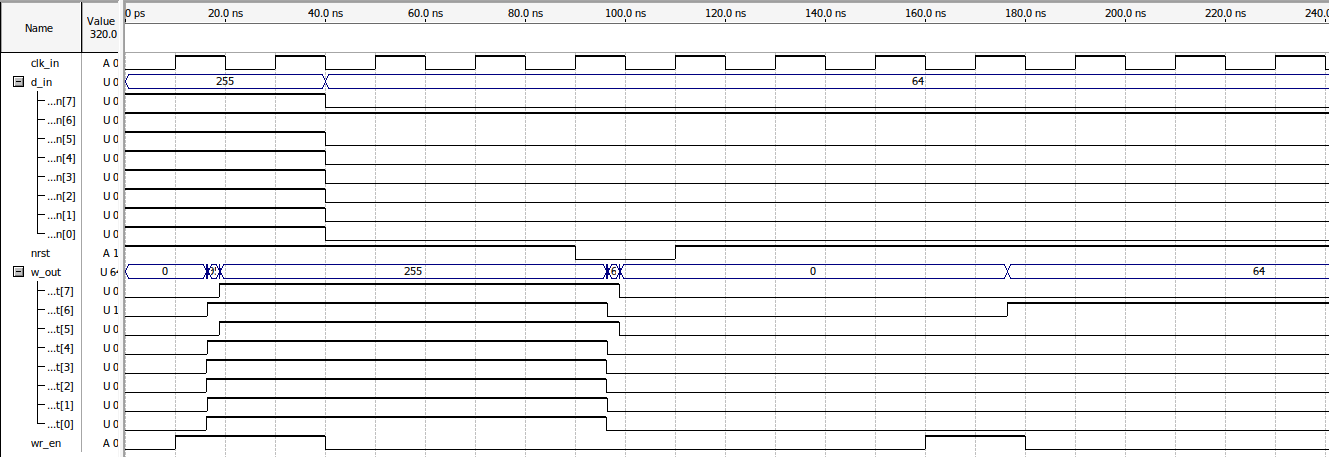
\includegraphics[width=15cm]{images/w_reg.png}
    \caption{Simulação bloco w\_reg}
\end{center}
\end{figure}

\newpage

\section{fsr\_reg}

O registrador FSR é um registrador semelhante ao implementado anteriormente. A principal diferença entre os dois está na presença de um sistema de endereçamento, e de duas entradas binárias independentes para habilitação da escrita e da leitura. Os requisitos são descritos na tabela abaixo.

\begin{table}[ht]
    \begin{center}
        \begin{tabular}{|c|c|c|c|}
            \hline
            Nome & Tamanho & Tipo & Descrição\\
            \hline
            nrst & 1 bit & \textit{Input} & Entrada de \textit{reset} assíncrono.\\
            \hline
            clk\_in & 1 bit & \textit{Input} & Entrada de \textit{clock}.\\
            \hline
            abus\_in & 9 bit & \textit{Input} & Entrada de enderençamento.\\
            \hline
            dbus\_in & 8 bits & \textit{Input} & Entrada de dados para escrita.\\
            \hline
            wr\_en & 1 bit & \textit{Input} & Entrada de habilitação de escrita.\\
            \hline
            rd\_en & 1 bit & \textit{Input} & Entrada de habilitação de leitura.\\
            \hline
            dbus\_out & 8 bits & \textit{Output} & Saída de dados hailitada por rd\_en.\\
            \hline
        \end{tabular}
    \end{center}
    \caption{Entradas e Saídas de fsr\_reg}
\end{table}

\subsection{Implementação}

O registrador fsr\_reg foi implementado utilizando a linguagem VHDL.\\

O código na íntegra está abaixo:\\

\begin{lstlisting}[language=VHDL, caption={Código VHDL fsr\_reg}]
LIBRARY ieee;
USE ieee.std_logic_1164.all;
USE ieee.std_logic_unsigned.all;
USE ieee.numeric_std.all;

ENTITY fsr_reg IS
    PORT (
        -- Inputs
        nrst : IN STD_LOGIC;                            -- Reset
        clk_in: IN STD_LOGIC;                           -- Clock
        abus_in: IN STD_LOGIC_VECTOR(8 DOWNTO 0);       -- Enderecamento
        dbus_in: IN STD_LOGIC_VECTOR(7 DOWNTO 0);       -- Dados
        wr_en : IN STD_LOGIC;                           -- Enable escrita
        rd_en : IN STD_LOGIC;                           -- Enable leitura

        -- Outputs
        dbus_out : OUT STD_LOGIC_VECTOR(7 DOWNTO 0);    -- Dados
        fsr_out : OUT STD_LOGIC_VECTOR(7 DOWNTO 0)      -- Registrador
    );
END ENTITY;

ARCHITECTURE fsr_reg OF fsr_reg IS
    SIGNAL mem_reg: STD_LOGIC_VECTOR(7 DOWNTO 0);
BEGIN
    PROCESS (nrst, clk_in, mem_reg, abus_in, dbus_in)
    BEGIN
        IF nrst = '0' THEN                              -- reset
            mem_reg <= "00000000";
        ELSIF abus_in(6 DOWNTO 0) = "0000100" THEN
            IF RISING_EDGE(clk_in) THEN
                IF wr_en = '1' THEN                     -- write
                    mem_reg <= dbus_in;
                END IF;
            END IF;
        END IF;
    END PROCESS;

    dbus_out <= mem_reg WHEN rd_en = '1' ELSE "ZZZZZZZZ"; -- read
    fsr_out <= mem_reg;
END fsr_reg;    
\end{lstlisting}

\subsection{Simulação}

Para testar nosso código VHDL e certificar-nos de que nosso circuito funciona de maneira esperada, simulamos alguns casos de testes utilizando o software Quatus II.\\

Os testes realizados foram os seguites:

\begin{enumerate}
    \item Escrita com enderaçamento incorreto (diferente de XX0000100).
    \begin{itemize}
        \item \textbf{Comportamento esperado:}
        \begin{itemize}
            \item dbus\_out em alta impedância;
            \item fsr\_out sem alteração;
        \end{itemize}
    \end{itemize}
    
    \item Leitura habilitada e escrita desabilitada.
    \begin{itemize}
        \item \textbf{Comportamento esperado:}
        \begin{itemize}
            \item dbus\_out = frs\_out = último valor escrito;
        \end{itemize}
    \end{itemize}

    \item Leitura desabilitada e escrita habilitada.
    \begin{itemize}
        \item \textbf{Comportamento esperado:}
        \begin{itemize}
            \item dbus\_out em alta impendância;
            \item frs\_out = dbus\_in;
        \end{itemize}
    \end{itemize}

    \item \textit{Reset} com leitura habilitada.
    \begin{itemize}
        \item \textbf{Comportamento esperado:}
        \begin{itemize}
            \item dbus\_out = frs\_out = ``0b00000000'';
        \end{itemize}
    \end{itemize}
\end{enumerate}

\begin{figure}[ht]
    \begin{center}
        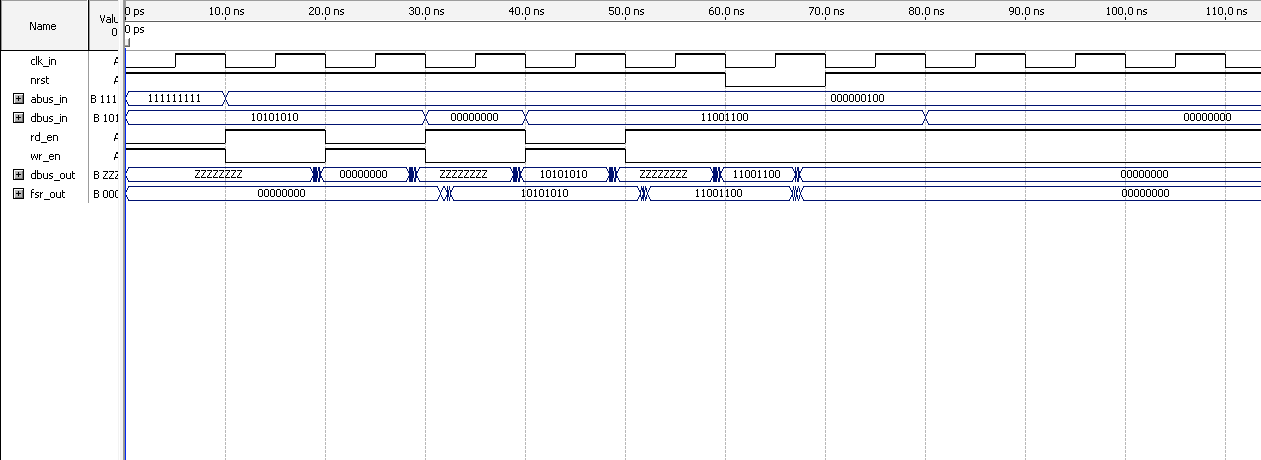
\includegraphics[width=15cm]{images/fsr_reg.png}
        \caption{Simulação fsr\_reg}
\end{center}
\end{figure}

\newpage

\section{status\_reg}

O status é um registrador semelhante ao implementado anteriormente. A diferença esta na presença de sinais de entrada e saída para controlar bits específicos. Assim como o anterior, existe um sistema de endereçamento que deve ser conferido para alterar o registrador.\\

As entradas e saídas do circuito são descritas na tabela a baixo:\\

\begin{table}[ht]
    \begin{center}
        \begin{tabular}{|c|c|c|c|}
            \hline
            Nome & Tamanho & Tipo & Descrição\\
            \hline
            nrst & 1 bit & \textit{Input} & Entrada de \textit{reset} assíncrono.\\
            \hline
            clk\_in & 1 bit & \textit{Input} & Entrada de \textit{clock}.\\
            \hline
            abus\_in & 9 bit & \textit{Input} & Entrada de enderençamento.\\
            \hline
            dbus\_in & 8 bits & \textit{Input} & Entrada de dados para escrita.\\
            \hline
            wr\_en & 1 bit & \textit{Input} & Entrada de habilitação de escrita.\\
            \hline
            rd\_en & 1 bit & \textit{Input} & Entrada de habilitação de leitura.\\
            \hline
            z\_in & 1 bit & \textit{Input} & Entrada de dado para escrita no bit 2 do registrador.\\
            \hline
            dc\_in & 1 bit & \textit{Input} & Entrada de dado para escrita no bit 1 do registrador.\\
            \hline
            c\_in & 1 bit & \textit{Input} & Entrada de dado para escrita no bit 0 do registrador.\\
            \hline
            z\_wr\_en & 1 bit & \textit{Input} & Entrada para habilitação da escrita no bit 2 do registrador.\\
            \hline
            dc\_wr\_en & 1 bit & \textit{Input} & Entrada para habilitação da escrita no bit 1 do registrador.\\
            \hline
            c\_wr\_en & 1 bit & \textit{Input} & Entrada para habilitação da escrita no bit 0 do registrador.\\
            \hline
            dbus\_out & 8 bits & \textit{Output} & Saída de dados hailitada por rd\_en.\\
            \hline
            irp\_out & 1 bit & \textit{Output} & Saída correspondente ao bit 7 do registrador.\\
            \hline
            rp\_out & 2 bits & \textit{Output} & Saída correspondente aos bits 6 e 5 do registrador.\\
            \hline
            z\_out & 1 bit & \textit{Output} & Saída correspondente ao bit 2 do registrador.\\
            \hline\
            dc\_out & 1 bit & \textit{Output} & Saída correspondente ao bit 1 do registrador.\\
            \hline
            c\_out & 1 bit & \textit{Output} & Saída correspondente ao bit 0 do registrador.\\
            \hline
        \end{tabular}
    \end{center}
    \caption{Entradas e Saídas de status\_reg}
\end{table}

\subsection{Implementação}

O status\_reg foi implementado utilizando a linguagem VHDL.\\

O código na íntegra está abaixo:\\

\begin{lstlisting}[language=VHDL, caption={Código VHDL status\_reg}]
LIBRARY ieee;
USE ieee.std_logic_1164.all;
USE ieee.std_logic_unsigned.all;
USE ieee.numeric_std.all;

ENTITY status_reg IS
    PORT (
        -- Inputs
        nrst: IN STD_LOGIC;                             -- Reset
        clk_in: IN STD_LOGIC;                           -- Clock
        abus_in: IN STD_LOGIC_VECTOR(8 DOWNTO 0);       -- Enderecamento
        dbus_in: IN STD_LOGIC_VECTOR(7 DOWNTO 0);       -- Dados
        wr_en: IN STD_LOGIC;                            -- Enable escrita
        rd_en: IN STD_LOGIC;                            -- Enable leitura
        z_in: IN STD_LOGIC;                             -- Dados bit 2
        dc_in: IN STD_LOGIC;                            -- Dados bit 1
        c_in: IN STD_LOGIC;                             -- Dados bit 0
        z_wr_en: IN STD_LOGIC;                          -- Enable escrita bit 2
        dc_wr_en: IN STD_LOGIC;                         -- Enable escrita bit 1
        c_wr_en: IN STD_LOGIC;                          -- Enable escrita bit 0

        -- Outputs
        dbus_out: OUT STD_LOGIC_VECTOR(7 DOWNTO 0);     -- Dados
        irp_out: OUT STD_LOGIC;                         -- Dados bit 7
        rp_out: OUT STD_LOGIC_VECTOR(1 DOWNTO 0);       -- Dados bit 6 e 5
        z_out: OUT STD_LOGIC;                           -- Dados bit 2
        dc_out: OUT STD_LOGIC;                          -- Dados bit 1
        c_out: OUT STD_LOGIC                            -- Dados bit 0
    );  
END ENTITY;

ARCHITECTURE status_reg OF status_reg IS
    SIGNAL mem_reg: STD_LOGIC_VECTOR(7 downto 0);
BEGIN
    PROCESS(nrst, clk_in, mem_reg, wr_en, z_in, dc_in, c_in)
    BEGIN
        IF nrst = '0' THEN                              -- reset
            mem_reg <= "00000000";
        ELSIF RISING_EDGE(clk_in) THEN
            IF wr_en = '1' AND abus_in(6 DOWNTO 0) = "0000011" THEN
                mem_reg <= dbus_in;                     -- write
            END IF;
            IF z_wr_en = '1' THEN
                mem_reg(2) <= z_in;                                     
            END IF;
            IF dc_wr_en = '1' THEN
                mem_reg(1) <= dc_in;
            END IF;
            IF c_wr_en = '1' THEN
                mem_reg(0) <= c_in;
            END IF;
        END IF;
    END PROCESS;
    
    -- output
    dbus_out <= mem_reg WHEN rd_en = '1' AND abus_in(6 DOWNTO 0) = "0000011" ELSE "ZZZZZZZZ";
    irp_out <= mem_reg(7);
    rp_out <= mem_reg(6 DOWNTO 5);
    z_out <= mem_reg(2);
    dc_out <= mem_reg(1);
    c_out <= mem_reg(0);
END status_reg;
\end{lstlisting}

\subsection{Simulação}

Para testar nosso código VHDL e certificar-nos de que nosso circuito funciona de maneira esperada, simulamos alguns casos de testes utilizando o software Quatus II.\\

Os testes realizados foram os seguites:

\begin{enumerate}
    \item Escrita com enderaçamento incorreto (diferente de ``0bXX0000011).
    \begin{itemize}
        \item \textbf{Comportamento esperado:}
        \begin{itemize}
            \item dbus\_out em alta impedância;
            \item rp\_out = ``0b00''
            \item irp\_out = z\_out = dc\_out = c\_out = ``0b0''
        \end{itemize}
    \end{itemize}
    
    \item Leitura desabilitada e escrita habilitada;
    \begin{itemize}
        \item dbus\_in = ``0b01011000''.\
        \item z\_in = dc\_in = c\_in = 1;
        \item z\_wr\_en = dc\_wr\_en = c\_wr\_en = 0;
        \item \textbf{Comportamento esperado:}
        \begin{itemize}
            \item dbus\_out em alta impendância;
            \item rp\_out = ``10b''
            \item irp\_out = z\_out = dc\_out = c\_out = ``0b0''
        \end{itemize}
    \end{itemize}

    \item Leitura habilitada e escrita desabilitada.
    \begin{itemize}
        \item Valor salvo = ``0b01011000''.
        \item \textbf{Comportamento esperado:}
        \begin{itemize}
            \item dbus\_out = ``0b01011000'';
            \item rp\_out = ``10b''
            \item irp\_out = z\_out = dc\_out = c\_out = ``0b0''
        \end{itemize}
    \end{itemize}

    \item Leitura desabilitada e escrita habilitada;
    \begin{itemize}
        \item dbus\_in = ``0b10100000''.
        \item z\_in = dc\_in = c\_in = 1;
        \item z\_wr\_en = dc\_wr\_en = c\_wr\_en = 1;
        \item \textbf{Comportamento esperado:}
        \begin{itemize}
            \item dbus\_out em alta impendância;
            \item rp\_out = ``01b''
            \item irp\_out = z\_out = dc\_out = c\_out = ``0b1''
        \end{itemize}
    \end{itemize}

    \item Leitura habilitada e escrita desabilitada.
    \begin{itemize}
        \item Valor salvo = ``0b10100111''.
        \item \textbf{Comportamento esperado:}
        \begin{itemize}
            \item dbus\_out = ``0b10100111'';
            \item rp\_out = ``10b''
            \item irp\_out = z\_out = dc\_out = c\_out = ``0b1''
        \end{itemize}
    \end{itemize}

    \item \textit{Reset} com leitura habilitada.
    \begin{itemize}
        \item \textbf{Comportamento esperado:}
        \begin{itemize}
            \item dbus\_out = ``0b00000000'';
            \item rp\_out = ``00b''
            \item irp\_out = z\_out = dc\_out = c\_out = ``0b0''
        \end{itemize}
    \end{itemize}
\end{enumerate}

\begin{figure}[ht]
    \begin{center}
        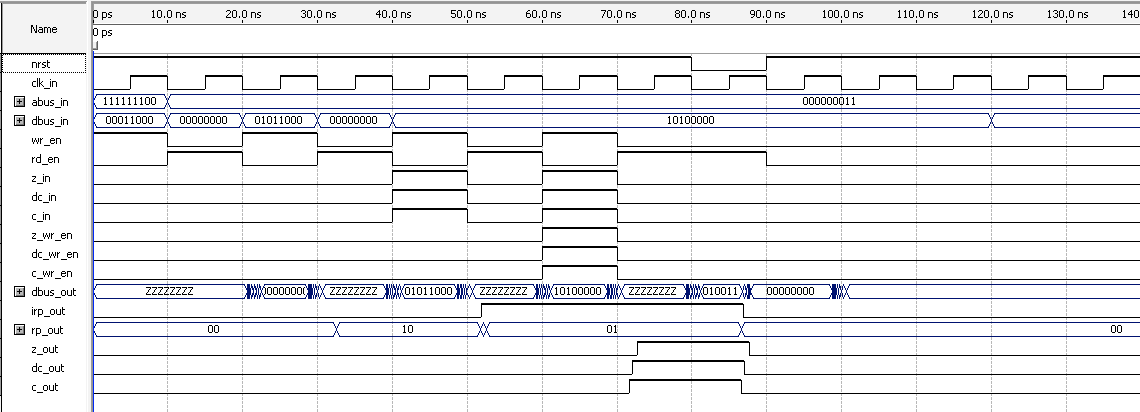
\includegraphics[width=15cm]{images/status.png}
        \caption{Simulação status\_reg}
\end{center}
\end{figure}

\newpage

\section{stack}

O bloco \textbf{stack} é um conjunto de 8 registradores de 13 bits. As operações de \textit{push} e \textit{pop} adicionam e removem dados da pilha, respectivamente.\\

As entradas e saídas deste bloco estão descritas na tabela abaixo:\\

\begin{table}[ht]
    \begin{center}
        \begin{tabular}{|c|c|c|c|}
            \hline
            Nome & Tamanho & Tipo & Descrição\\
            \hline
            nrst & 1 bit & \textit{Input} & Entrada de \textit{reset} assíncrono.\\
            \hline
            clk\_in & 1 bit & \textit{Input} & Entrada de \textit{clock}.\\
            \hline
            stack\_in & 13 bit & \textit{Input} & Entrada de dados para a pilha.\\
            \hline
            stack\_push & 1 bit & \textit{Input} & Entrada de habilitação para colocar valores na pilha.\\
            \hline
            stack\_pop & 1 bit & \textit{Input} & Entrada de habilitação para retirar valores da pilha.\\
            \hline
            stack\_out & 13 bits & \textit{Output} & Saída correspondente à primeira posição da pilha.\\
            \hline
        \end{tabular}
    \end{center}
    \caption{Entradas e Saídas do bloco stack}
\end{table}

\subsection{Implementação}

O bloco stack foi implementado utilizando a linguagem VHDL.\\

O código na íntegra está abaixo:\\

\begin{lstlisting}[language=VHDL, caption={Código VHDL stack}]
LIBRARY ieee;
USE ieee.std_logic_1164.all;
USE ieee.std_logic_unsigned.all;
USE ieee.numeric_std.all;

ENTITY stack IS
    PORT (
        -- Inputs
        nrst: IN STD_LOGIC;                             -- Reset
        clk_in: IN STD_LOGIC;                           -- Clock
        stack_in: IN STD_LOGIC_VECTOR(12 DOWNTO 0);     -- Dados
        stack_push: IN STD_LOGIC;                       -- Enable push op
        stack_pop: IN STD_LOGIC;                        -- Enable pop op
        
        -- Outputs
        stack_out: OUT STD_LOGIC_VECTOR(12 DOWNTO 0)    -- Stack output
    );
END ENTITY;

ARCHITECTURE stack OF stack IS
    SIGNAL mem_reg1, mem_reg2, mem_reg3, mem_reg4, mem_reg5, mem_reg6, mem_reg7, mem_reg8 : STD_LOGIC_VECTOR(12 DOWNTO 0);
BEGIN
    PROCESS(nrst, clk_in, stack_push, stack_pop)
    BEGIN
        IF nrst = '0' THEN                              -- registradores
            mem_reg1 <= "0000000000000";
            mem_reg2 <= "0000000000000";
            mem_reg3 <= "0000000000000";
            mem_reg4 <= "0000000000000";
            mem_reg5 <= "0000000000000";
            mem_reg6 <= "0000000000000";
            mem_reg7 <= "0000000000000";
            mem_reg8 <= "0000000000000";
        ELSIF RISING_EDGE(clk_in) THEN
			stack_out <= "0000000000000";
            IF stack_pop = '1' THEN                     -- pop
                stack_out <= mem_reg1;                  -- output
                mem_reg1 <= mem_reg2;
                mem_reg2 <= mem_reg3;
                mem_reg3 <= mem_reg4;
                mem_reg4 <= mem_reg5;
                mem_reg5 <= mem_reg6;
                mem_reg6 <= mem_reg7;
                mem_reg7 <= mem_reg8;
                mem_reg8 <= "0000000000000";
            ELSIF stack_push = '1' THEN                 -- push
                mem_reg8 <= mem_reg7;
                mem_reg7 <= mem_reg6;
                mem_reg6 <= mem_reg5;
                mem_reg5 <= mem_reg4;
                mem_reg4 <= mem_reg3;
                mem_reg3 <= mem_reg2;
                mem_reg2 <= mem_reg1;
                mem_reg1 <= stack_in; 
            END IF;
        END IF;
    END PROCESS;
END stack;
\end{lstlisting}

\subsection{Simulação}

Para testar nosso código VHDL e certificar-nos de que nosso circuito funciona de maneira esperada, simulamos alguns casos de testes utilizando o software Quatus II.\\

Os testes realizados foram os seguites:

\begin{enumerate}
    \item \textit{Push} até pilha cheia.
    \begin{itemize}
        \item stack\_in: Sequência de ``0'' à ``7'';
        \item stack\_push = ``1'';
        \item stack\_pop = ``0'';
        \item \textbf{Comportamento esperado:}
        \begin{itemize}
            \item stack\_out = ``0'';
        \end{itemize}
    \end{itemize}

    \item \textit{Pop} até pilha vazia.
    \begin{itemize}
        \item stack\_push = ``0'';
        \item stack\_pop = ``1'';
        \item \textbf{Comportamento esperado:}
        \begin{itemize}
            \item stack\_out = Sequência de ``7'' à ``0'';
        \end{itemize}
    \end{itemize}

    \item \textit{Push} até \textit{Stack Overvlow}.
    \begin{itemize}
        \item stack\_in: Sequência de ``0'' à ``9'';
        \item stack\_push = ``1'';
        \item stack\_pop = ``0'';
        \item \textbf{Comportamento esperado:}
        \begin{itemize}
            \item stack\_out = ``0'';
        \end{itemize}
    \end{itemize}

    \item \textit{Pop} até \textit{Stack Underflow}.
    \begin{itemize}
        \item stack: Sequência de ``9'' à ``2'';
        \item stack\_push = ``0'';
        \item stack\_pop = ``1'';
        \item \textbf{Comportamento esperado:}
        \begin{itemize}
            \item stack\_out = Sequência de ``9'' à ``2'', depois, ``0'';
        \end{itemize}
    \end{itemize}

    \item \textit{Push} e \textit{Pop} simultâneo.
    \begin{itemize}
        \item stack: ``1'';
        \item stack\_push = ``1'';
        \item stack\_pop = ``1'';
        \item \textbf{Comportamento esperado:}
        \begin{itemize}
            \item Preferência do \textit{pop}.
            \item stack\_out = ``1'', depois, ``0'';
        \end{itemize}
    \end{itemize}
\end{enumerate}

\begin{figure}[ht]
    \begin{center}
        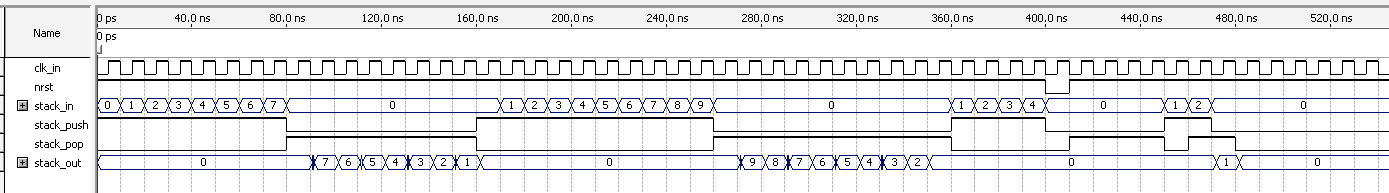
\includegraphics[width=15cm]{images/stack.png}
        \caption{Simulação bloco stack}
\end{center}
\end{figure}

\newpage

\section{pc\_reg}

O bloco pc\_reg controla o registrados pc de um processador. Possui operações para incremento de endereço, \textit{load}, \textit{reset} e escrita, bem como operações de \textit{push} e \textit{pop} adicionam e removem o valor corrente de pc à uma pilha pilha.\\

As entradas e saídas deste bloco estão descritas na tabela abaixo:\\

\begin{table}[ht]
    \begin{center}
        \begin{tabular}{|c|c|c|c|}
            \hline
            Nome & Tamanho & Tipo & Descrição\\
            \hline
            nrst & 1 bit & \textit{Input} & Entrada de \textit{reset} assíncrono.\\
            \hline
            clk\_in & 1 bit & \textit{Input} & Entrada de \textit{clock}.\\
            \hline
            aadr\_in & 11 bits & \textit{Input} & Entrada de dados para carga no registrador PC.\\
            \hline
            abus\_in & 9 bits & \textit{Input} & Entrada de endereçamento para PCL e para o registrador PCLATH.\\
            \hline
            dbus\_in & 8 bits & \textit{Input} & Entrada de dados para escrita em PCL e PCLATH.\\
            \hline
            inc\_pc & 1 bit & \textit{Input} & Entrada de habilitação para incremento.\\
            \hline
            load\_pc & 1 bit & \textit{Input} & Entrada de habilitação para carga.\\
            \hline
            wr\_en & 1 bit & \textit{Input} & Entrada de habilitação para escrita nos registradores.\\
            \hline
            rd\_en & 1 bit & \textit{Input} & Entrada de habilitação para leitura dos registradores.\\
            \hline
            stack\_push & 1 bit & \textit{Input} & Entrada de habilitação para colocar valores na pilha.\\
            \hline
            stack\_pop & 1 bit & \textit{Input} & Entrada de habilitação para retirar valores da pilha.\\
            \hline
            nextpc\_out & 13 bits & \textit{Output} & Saída do valor a ser carregado no contador.\\
            \hline
            dbus\_out & 8 bits & \textit{Output} & Saída de dados lidos com endereçamento por abus\_in.\\
            \hline
        \end{tabular}
    \end{center}
    \caption{Entradas e Saídas do bloco pc\_reg}
\end{table}

\subsection{Implementação}

O bloco pc\_reg foi implementado utilizando a linguagem VHDL.\\

O código na íntegra está abaixo:\\

\begin{lstlisting}[language=VHDL, caption={Código VHDL pc\_reg}]
LIBRARY ieee;
USE ieee.std_logic_1164.all;
USE ieee.std_logic_unsigned.all;
USE ieee.numeric_std.all;

ENTITY pc_reg IS
    PORT (
        -- Inputs
        nrst: IN STD_LOGIC;                             -- Reset
        clk_in: IN STD_LOGIC;                           -- Clock
        addr_in: IN STD_LOGIC_VECTOR(10 DOWNTO 0);      -- Dados
        abus_in: IN STD_LOGIC_VECTOR(8 DOWNTO 0);       -- Enderecamento PCL e PCLATH
        dbus_in: IN STD_LOGIC_VECTOR(7 DOWNTO 0);       -- Dados PCL e PCLATH
        inc_pc: IN STD_LOGIC;                           -- Enable incremento.
        load_pc: IN STD_LOGIC;                          -- Enable carga.
        wr_en: IN STD_LOGIC;                            -- Enable escrita.
        rd_en: IN STD_LOGIC;                            -- Enable leitura.
        stack_push: IN STD_LOGIC;                       -- Enable push op
        stack_pop: IN STD_LOGIC;                        -- Enable pop op

        -- Outputs
        nextpc_out: OUT STD_LOGIC_VECTOR(12 DOWNTO 0);  -- Contador
        dbus_out: OUT STD_LOGIC_VECTOR(7 DOWNTO 0)      -- Dados
    );
END ENTITY;

ARCHITECTURE pc_reg OF pc_reg IS
    SIGNAL stack_reg1, stack_reg2, stack_reg3, stack_reg4, stack_reg5, stack_reg6, stack_reg7, stack_reg8 : STD_LOGIC_VECTOR(12 DOWNTO 0);
    SIGNAL stack_popped: STD_LOGIC_VECTOR(12 DOWNTO 0);
    SIGNAL pc: STD_LOGIC_VECTOR(12 DOWNTO 0);
    SIGNAL lath_pc: STD_LOGIC_VECTOR(7 DOWNTO 0);
    SIGNAL nextpc: STD_LOGIC_VECTOR(12 DOWNTO 0);
BEGIN

    -- Stack
    PROCESS(nrst, clk_in, stack_push, stack_pop, stack_popped)
    BEGIN
        IF nrst = '0' THEN
            stack_reg1 <= "0000000000000";
            stack_reg2 <= "0000000000000";
            stack_reg3 <= "0000000000000";
            stack_reg4 <= "0000000000000";
            stack_reg5 <= "0000000000000";
            stack_reg6 <= "0000000000000";
            stack_reg7 <= "0000000000000";
            stack_reg8 <= "0000000000000";
        ELSIF RISING_EDGE(clk_in) THEN
            IF stack_pop = '1' THEN
                stack_popped <= stack_reg1;
                stack_reg1 <= stack_reg2;
                stack_reg2 <= stack_reg3;
                stack_reg3 <= stack_reg4;
                stack_reg4 <= stack_reg5;
                stack_reg5 <= stack_reg6;
                stack_reg6 <= stack_reg7;
                stack_reg7 <= stack_reg8;
                stack_reg8 <= "0000000000000";
            ELSIF stack_push = '1' THEN
                stack_reg8 <= stack_reg7;
                stack_reg7 <= stack_reg6;
                stack_reg6 <= stack_reg5;
                stack_reg5 <= stack_reg4;
                stack_reg4 <= stack_reg3;
                stack_reg3 <= stack_reg2;
                stack_reg2 <= stack_reg1;
                stack_reg1 <= pc; 
            END IF;
        END IF;
    END PROCESS;

    -- logica combinacional para nextpc
    PROCESS(stack_pop, inc_pc, load_pc, wr_en, abus_in, pc, addr_in, lath_pc, stack_popped, dbus_in)
    BEGIN
        IF stack_pop = '1' THEN
            nextpc <= stack_popped;
        ELSIF inc_pc = '1' THEN
            nextpc <= pc + 1;
        ELSIF load_pc = '1' THEN
            nextpc(10 DOWNTO 0) <= addr_in;
            nextpc(12 DOWNTO 11) <= lath_pc(4 DOWNTO 3);
        ELSIF wr_en = '1' AND abus_in(6 DOWNTO 0) = "0000010" THEN
            nextpc <= lath_pc(4 DOWNTO 0) & dbus_in;
        ELSE
            nextpc <= pc;
        END IF;
        
        nextpc_out <= nextpc;
    END PROCESS;

    -- logica sequencial para PC_reg
    PROCESS(clk_in, nrst, pc, nextpc)
    BEGIN
        IF RISING_EDGE(clk_in) THEN
            pc <= nextpc;
        END IF;

        IF nrst = '0' THEN
            pc <= "0000000000000";
        END IF;
    END PROCESS;

    -- logica sequencial para PCLATH
    PROCESS(clk_in, nrst, wr_en, abus_in)
    BEGIN
        IF RISING_EDGE(clk_in) THEN
            IF wr_en = '1' AND abus_in(6 DOWNTO 0) = "0001010" THEN
                lath_pc <= dbus_in;
            END IF;
        END IF;
        
        IF nrst = '0' THEN
            lath_pc <= "00000000";
        END IF;
    END PROCESS;

    -- logica combinacional para dbus_out
    PROCESS(clk_in, rd_en, abus_in, lath_pc, pc)
    BEGIN
        IF abus_in(6 DOWNTO 0) = "0001010" AND rd_en = '1' THEN
            dbus_out <= lath_pc(7 DOWNTO 0);
        ELSIF abus_in(6 DOWNTO 0) = "0000010" AND rd_en = '1' THEN
            dbus_out <= pc(7 DOWNTO 0);
        ELSE
            dbus_out <= "ZZZZZZZZ";
        END IF;
    END PROCESS;

END pc_reg;
\end{lstlisting}

\subsection{Simulação}

Para testar nosso código VHDL e certificar-nos de que nosso circuito funciona de maneira esperada, simulamos alguns casos de testes utilizando o software Quatus II.\\

Os testes realizados foram os seguites:

\begin{enumerate}
    \item Incremento de PC (4x).
    \begin{itemize}
        \item inc\_pc: \textit{High} (4x);
        \item \textbf{Comportamento esperado:}
        \begin{itemize}
            \item nextpc\_out: Sequência de ``0x1'' à ``0x4'';
            \item dbus\_out: Alta impedância;
        \end{itemize}
    \end{itemize}

    \item \textit{Reset} do PC.
    \begin{itemize}
        \item nrst: \textit{High};
        \item \textbf{Comportamento esperado:}
        \begin{itemize}
            \item nextpc\_out: ``0x00'';
            \item dbus\_out: Alta impedância;
        \end{itemize}
    \end{itemize}

    \item Empilhamento e Desempilhamento de PC (``0x0'' e ``0x2'').
    \begin{itemize}
        \item stack\_push: \textit{High} (2x) e \textit{low} (2x);
        \item stack\_pop: \textit{Low} (2x) e \textit{high} (2x);
        \item \textbf{Comportamento esperado:}
        \begin{itemize}
            \item nextpc\_out: ``0x02'' e ``0x00'', nesta ordem;
            \item dbus\_out: Alta impedância;
        \end{itemize}
    \end{itemize}

    \item Escrita e leitura de PCL (``0x0'' e ``0x2'').
    \begin{itemize}
        \item abus\_in: ``0x002'';
        \item dbus\_in: ``0x0A''
        \item wr\_en: \textit{High} na escrita. \textit{low} na leitura;
        \item rd\_en: \textit{Low} na escrita. \textit{high} na leitura;
        \item \textbf{Comportamento esperado:}
        \begin{itemize}
            \item nextpc\_out: ``0x?0A'';
            \item dbus\_out: ``0x0A'';
        \end{itemize}
    \end{itemize}
    
    \item Carregamento de endereço.
    \begin{itemize}
        \item addr\_in: ``0x3AB'';
        \item load\_pc: \textit{High};
        \item \textbf{Comportamento esperado:}
        \begin{itemize}
            \item nextpc\_out: ``0x3AB'';
            \item dbus\_out: Alta impedância;
        \end{itemize}
    \end{itemize}

    \item Escrita e leitura de PCLATH (``0x0'' e ``0x2'').
    \begin{itemize}
        \item abus\_in: ``0x00A'';
        \item dbus\_in: ``0x18'';
        \item wr\_en: \textit{High} na escrita. \textit{low} na leitura;
        \item rd\_en: \textit{Low} na escrita. \textit{high} na leitura;
        \item \textbf{Comportamento esperado:}
        \begin{itemize}
            \item nextpc\_out: ``0x?18'';
            \item dbus\_out: ``0x0A'';
        \end{itemize}
    \end{itemize}
\end{enumerate}

\begin{figure}[ht]
    \begin{center}
        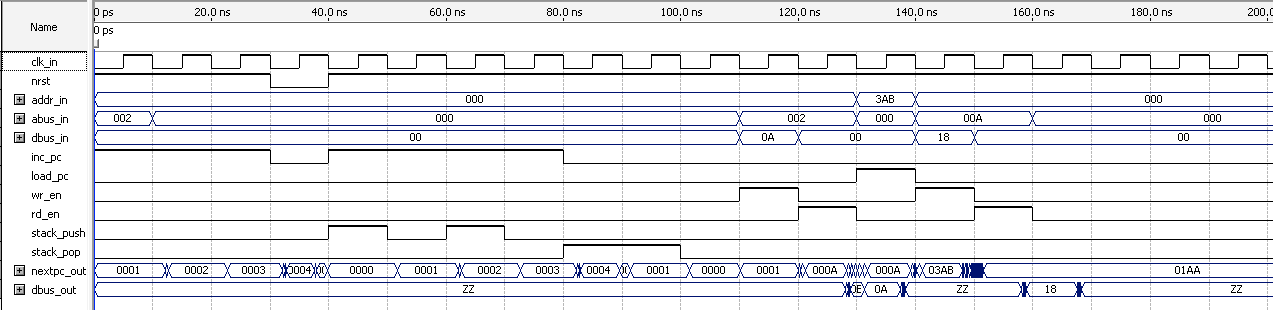
\includegraphics[width=15cm]{images/pc_reg.png}
        \caption{Simulação bloco pc\_reg}
\end{center}
\end{figure}

\section{Conclusão}

A implementação de registradores através de liguagens de descrição de hardware, como a VHDL, são maneiras poderosas de construir circuitos computacionais de maneira menos complexa e mais rápida.

Apesar de parecerem ``simples'' à primeira vista, sua implementação possuem nuancias que exigem a atenção do engenheiro, e testes exaustivos para certificar que funcionam como deveriam.

Neste trabalho prático, aprendemos como construir registradores e pilhas para auxiliar a contrução de nossos circuitos computacionais, utilizando conhecimentos da prática anterior e novas técnicas, como a utilização do ``PROCESS'', que permite a execução de trechos sequenciais no nosso circuito, e a tuilização do \textit{clock},  que permite a sincronização de rotinas no nosso cicuito.

Com os circuitos implementados, estamos mais confiantes nas nossas capacidades, e estamos um passo mais perto de implementar circuitos mais complexos como controladores e processadores.

\end{document}